\documentclass[12pt]{article}

\usepackage{amssymb,amsmath,amsfonts,eurosym,geometry,ulem,graphicx,caption,color,setspace,sectsty,comment,footmisc,caption,natbib,pdflscape,subfigure,array,hyperref}
\usepackage{multirow,booktabs}

\normalem

\onehalfspacing
\newtheorem{theorem}{Theorem}
\newtheorem{corollary}[theorem]{Corollary}
\newtheorem{proposition}{Proposition}
\newenvironment{proof}[1][Proof]{\noindent\textbf{#1.} }{\ \rule{0.5em}{0.5em}}

\newtheorem{hyp}{Hypothesis}
\newtheorem{subhyp}{Hypothesis}[hyp]
\renewcommand{\thesubhyp}{\thehyp\alph{subhyp}}

\newcommand{\red}[1]{{\color{red} #1}}
\newcommand{\blue}[1]{{\color{blue} #1}}

\newcolumntype{L}[1]{>{\raggedright\let\newline\\arraybackslash\hspace{0pt}}m{#1}}
\newcolumntype{C}[1]{>{\centering\let\newline\\arraybackslash\hspace{0pt}}m{#1}}
\newcolumntype{R}[1]{>{\raggedleft\let\newline\\arraybackslash\hspace{0pt}}m{#1}}

\geometry{left=1.0in,right=1.0in,top=1.0in,bottom=1.0in}

\begin{document}

\begin{titlepage}
\title{Clustering Companies With Text}
\author{Gao Haocheng \and He Junjie}
\date{April 2020}
\maketitle
\begin{abstract}
\noindent The aim of this project is to develop an effective model to 
cluster the companies within financial market, so that the group systematic
risk and intra-group similarity can be better explained by the new clustering 
structure, compared with official classification by industries.\\
\noindent We tried revenue catagories text and introduction text disclosed in
the annual reports as inputs, BERT, word2vec, dot2vec, Latent semantic indexing with different layers 
as company vector processing schemes, and greedy cosine-similarity, k-Means, Gausian
Mixture Model, and Deep Embedding for Clustering model as clustering schemes. this
working paper introduces how we impletemented these models and discusses briefly 
on the results.\\
\vspace{0in}\\
\noindent\textbf{Keywords:} BERT, word2vec, dot2vec, Latent semantic indexing, cosine similarity, 
k-Means, Gausian Mixture Model, Deep Embedding for Clustering\\

\bigskip
\end{abstract}
\setcounter{page}{0}
\thispagestyle{empty}
\end{titlepage}
\pagebreak \newpage




\doublespacing


\section{The Vectorizing Models} \label{sec:the vectorizing models}

\section{The Clustering Models} \label{sec:the clustering models}

\subsection{Greedy Cosine Similarity}

For company vector as inputs, in order to derive the firm-to-firm network 
representation of our industries, we use the vectors $V_i$ and $V_j$ for 
a pair of firms i and j to calculate the company cosine similarity or 
the firm pairwise similarity score as follows: 

\begin{equation}
    Company\,Cosine\,Similarity\,_{i,j}=\left(V_i \cdot V_j\right)
\end{equation}

The network representation of firms is fully described by an $\left(N_t \cdot N_t\right)$ square 
matrix $M_t$ (i.e., a network), where an entry of this matrix for row i and column j 
is the Company Cosine Similarity for firms i and j defined above. The large 
number of words used in business descriptions ensures that the matrix Mt is not 
sparse and that its entries are unrestricted real numbers in the interval [0, 1]. 

To process product-wise revenue classification text, an additional step is conducted 
before computing company cosine similarity. In this case, each product text vector is 
fed to the model, first a product pairwise similarity score is calculated as follows: 

\begin{equation}
    Product\,Cosine\,Similarity\,_{ai,bj}=\left(P_{ai} \cdot P_{bj}\right)
\end{equation}

\noindent where $Product\,Cosine\,Similarity\,_{ai,bj}$ is the score of $P_{ai}$, the 
$i^{th}$ producth of company a, and $P_{bj}$, $j^{th}$ producth of company b.
Therefore we can calculate the firm pairwise similarity score as follows: 

\begin{equation}
    Company\,Cosine\,Similarity\,_{a,b}=
    \sum_{i=1,j=1}^{n,n}Product\,Cosine\,Similarity
    \,_{ai,bj}w_{ai}w_{bj}
\end{equation}

\noindent where $w_{ai}\,w_{bj}$ are the proportions of product i in company a's revenue and 
that of product j in company b's revenue, respectively.\\

The next stage of clustering \cite{NBERw15991} is conducted by taking the subsample of N single-segment firms. 
Then the industry classifications is initialized to have N industries, with each of the N firms 
residing within its own one-firm industry. Then is pairwise similarity for each unique pair of 
industries j and k, which is denoted as $I_{j,k}$.\\
To reduce the industry count to N-1 industries, we take the maximum pairwise industry similarity as follows:

\begin{equation}
    \max_{j,k,j\neq k} I_{j,k}
\end{equation}

The two industries with the highest similarity are then combined, reducing the industry count by one. 
This process is repeated until the number of industries reaches the desired number. Importantly, when 
two industries with $m_j$ and $m_k$ firms are combined, all industry similarities relative to the new 
industry must be recomputed. For a newly created industry l, for example, its similarity with respect 
to all other industries q is computed as the average firm pairwise similar- ity for all firm pairs in 
which one firm is in industry l and one in industry q as follows:

\begin{equation}
    I_{l,q}=\sum_{x=1}^{m_t}\sum_{y=1}^{m_q} \frac{S_{x,y}}{m_l \cdot m_q}
\end{equation}

Here, $S_{x,y}$ is the firm-level pairwise similarity between firm x in industry l and firm y in industry q.

\subsection{k-Means}

k-means clustering is a method of vector quantization, aiming to partition n observations into k clusters 
in which each observation belongs to the cluster with the nearest mean (cluster centers or cluster 
centroid), serving as a prototype of the cluster.
Given a set of observations $\{x_1, x_2, ..., x_n\}$, where each observation is a d-dimensional real vector, 
k-means clustering aims to partition the n observations into k sets $S = \{S_1, S_2, ..., S_k\}$ so as to 
minimize the inter cluster variance:

\begin{equation}
    \arg\min_s\sum_{i=1}^k\sum_{x\in S_i}||x-\mu_i||^2
\end{equation}

\subsection{Gaussian Mixture Model}

A mixture model is a probabilistic model that assumes all the data points are generated from a mixture of a 
finite number of certain different distributions with unknown parameters. One can think of mixture models as 
generalizing k-Means clustering to incorporate information about the covariance structure of the data as well 
as the centers of the latent factor. The probability density is defined as a linear function of densities of 
all these K distributions:

\begin{equation}
    p(X)=\sum_{k=1}^K\phi_k f_k(X|\mu_k,\Sigma_k)
\end{equation}

In the formula, the distribution function of $k^{th}$ cluster is characterized by distribution function $f_k$ 
with weights $\phi_k$, mean $\mu_k$ and covariance matrix $\Sigma_k$. For Gaussian Mixture Model, the 
probability density functions of all clusters are assumed to be Gaussian distribution.

\subsection{Deep Embedding for Clustering}

The Deep Embedding for Clustering (DEC) model is built upon the Stacked Autoencoder (SAE) model. 
Autoencoder is a kind of unsupervised learning structure that owns three layers: input layer, hidden layer, 
and output layer. The process of an autoencoder training consists of two parts: encoder and decoder. 
Encoder is used for mapping the input data into hidden representation, and decoder is referred to reconstructing 
input data from the hidden representation. Then the structure of SAEs is stacking autoencoders into hidden 
layers by an unsupervised layer-wise learning algorithm and then fine-tuned by a supervised method. The structure
of SAE is illustrated in Figure~\ref{fig:fullSAEmodel}.\\
After greedy layer-wise training, we concatenate all encoder layers followed by all decoder layers, in reverse 
layer-wise training order, to form a deep autoencoder and then finetune it to minimize reconstruction loss. The 
final result is a multilayer deep autoencoder with a bottleneck coding layer in the middle. We then discard the decoder
ayers and use the encoder layers as our initial mapping between the data space and the feature space, as shown in
Figure~\ref{fig:SAEmodel}.\cite{zabalza2016novel}

Following \citep{pmlr-v48-xieb16}, we then add a new clustering layer to iteratively refine the clusters by learning 
from their high confidence assignments with the help of an auxiliary target distribution. Specifically, the model 
is trained by matching the soft assignment to the target distribution. To this end, we define our objective as a 
Kullback-Leibler (KL) divergence loss between the soft assignments $q_i$ and the auxiliary distribution $p_i$ as follows:

\begin{equation}
    L=KL(P||Q)=\sum_i\sum_j p_{ij}log\frac{p_{ij}}{q_{ij}}
\end{equation}

\noindent where the soft assignments $q_i$ is defined as follows:

\begin{equation}
    q_{ij}=\frac{(1+||z_i-\mu_j||^2/\alpha)^{-\frac{\alpha+1}{2}}}{\sum_{j'}(1+||z_i-\mu_{j'}||^2/\alpha)^{-\frac{\alpha+1}{2}}}
\end{equation}

\noindent where $z_i$ are the embedding vectors of each companies, and $u_j$ are the centroids of each group j. 
Following \cite{pmlr-v48-xieb16}, we set $\alpha=1$ and the auxiliary distribution $p_i$ as:

\begin{equation}
    p_{ij}=\frac{q_{ij}^2/f_j}{\sum_{j'}q_{ij'}^2/f_{j'}}
\end{equation}

The overall structure and the hyper-parameters are shown as in Figure~\ref{fig:DECmodel}. The training scheme is:
\begin{enumerate}
    \item Pretrain the full SAE model and get the weights;
    \item Pretrain a baseline machine learning classifier (we use k-Means in this model);
    \item Construct the DEC model and load pretrain weights;
    \item Initialize the clustering layer to the k-Means centroids;
    \item Train the DEC model.
\end{enumerate}



\section{Data and Results} \label{sec:data and results}

The input data contains two parts: 1. the revenue breakdown by different products stated in the annual reports, 
including the text and the sales figures as of 31 December 2018; 2. the descriptive text about the operartion, 
the main products of the company; 3. the daily stock price of the corresponding companies in 2019.
The total sample size is 3801.\\
We evaluate each model by the following method: for each clustering of carried out by each model, feed each
the time series return of each company with respect to the mean return of the group in a naive linear model, 
then calculate the average regression R square, which serves as the indicator of the performance of the models.\\
The results are summarized in Table~\ref{tab:performance}

\section{Discussions} \label{sec:discussion}

\section{Conclusion} \label{sec:conclusion}

\clearpage

\onehalfspacing

\section*{Tables and Figures} \label{sec:tab}
\addcontentsline{toc}{section}{Tables}
\newcommand{\tabincell}[2]{\begin{tabular}{@{}#1@{}}#2\end{tabular}}
\begin{table}[h]
    \begin{center}
        \begin{tabular}{c|c|c|c|c|c|c}
            \toprule
            \multirow{2}*{Embedding}&\multicolumn{6}{c}{Clustering Models}\\
            \cline{2-7}
            &official&\tabincell{c}{greedy\\(prodduct-based)}&\tabincell{c}{greedy\\(company-based)}&k-Means&GMM&DEC\\
            \hline
            \tabincell{c}{BERT}&\multirow{4}*{0.3791}&&&&&\tabincell{c}{0.3425\\1 pooling layer}\\
            \cline{1-1}\cline{3-7}
            Bag of Words&&&&&&0.4139\\
            \cline{1-1}\cline{3-7}
            \tabincell{c}{dot to vec}&&&&&&\tabincell{c}{0.4240\\300 length}\\
            \cline{1-1}\cline{3-7}
            \tabincell{c}{LSI}&&&&&&\tabincell{c}{0.4100\\500 length}\\
            \bottomrule
            

        \end{tabular}
        \caption{The average R square performance of each model}
        \label{tab:performance}
    \end{center}
\end{table}


\begin{figure}[hp]
    \centering
    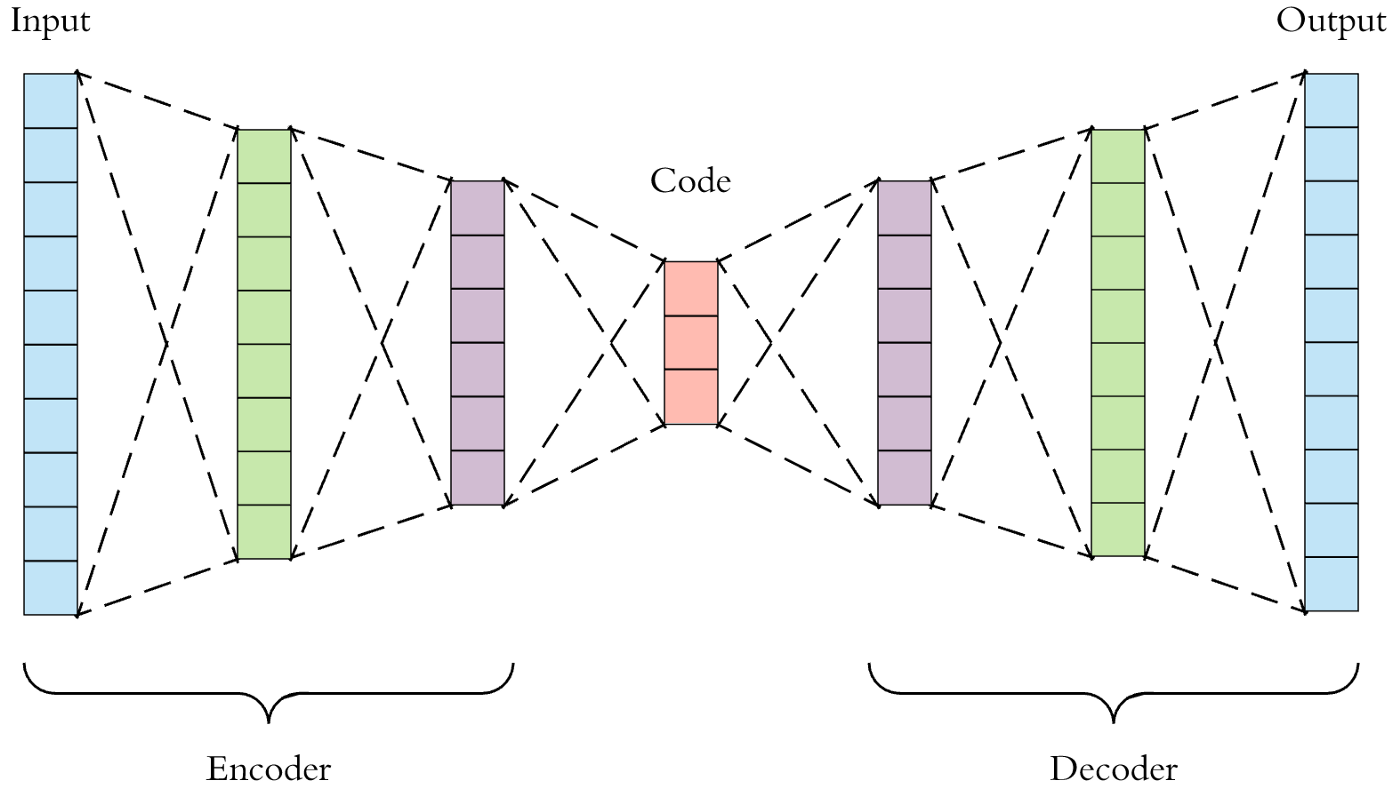
\includegraphics[width=.6\textwidth]{fig/fullSAEmodel.png}
    \caption{The Structure of a full SAE model, including encoder and decoder}
    \label{fig:fullSAEmodel}
\end{figure}

\begin{figure}[hp]
    \centering
    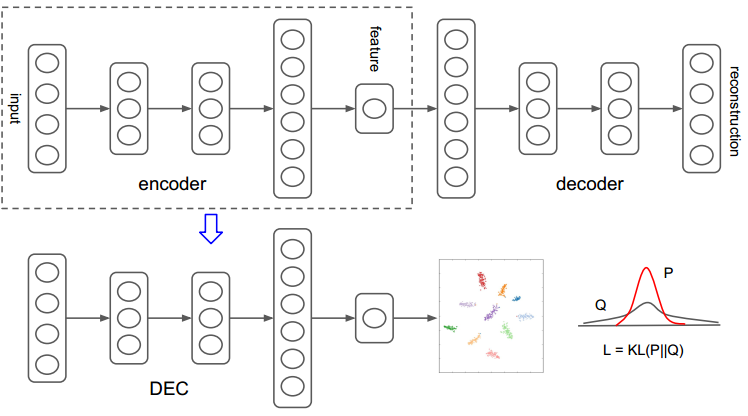
\includegraphics[width=.6\textwidth]{fig/deep-clustering-model.png}
    \caption{The Structure of an SAE model only considering encoder}
    \label{fig:SAEmodel}
\end{figure}

\begin{figure}[hp]
    \centering
    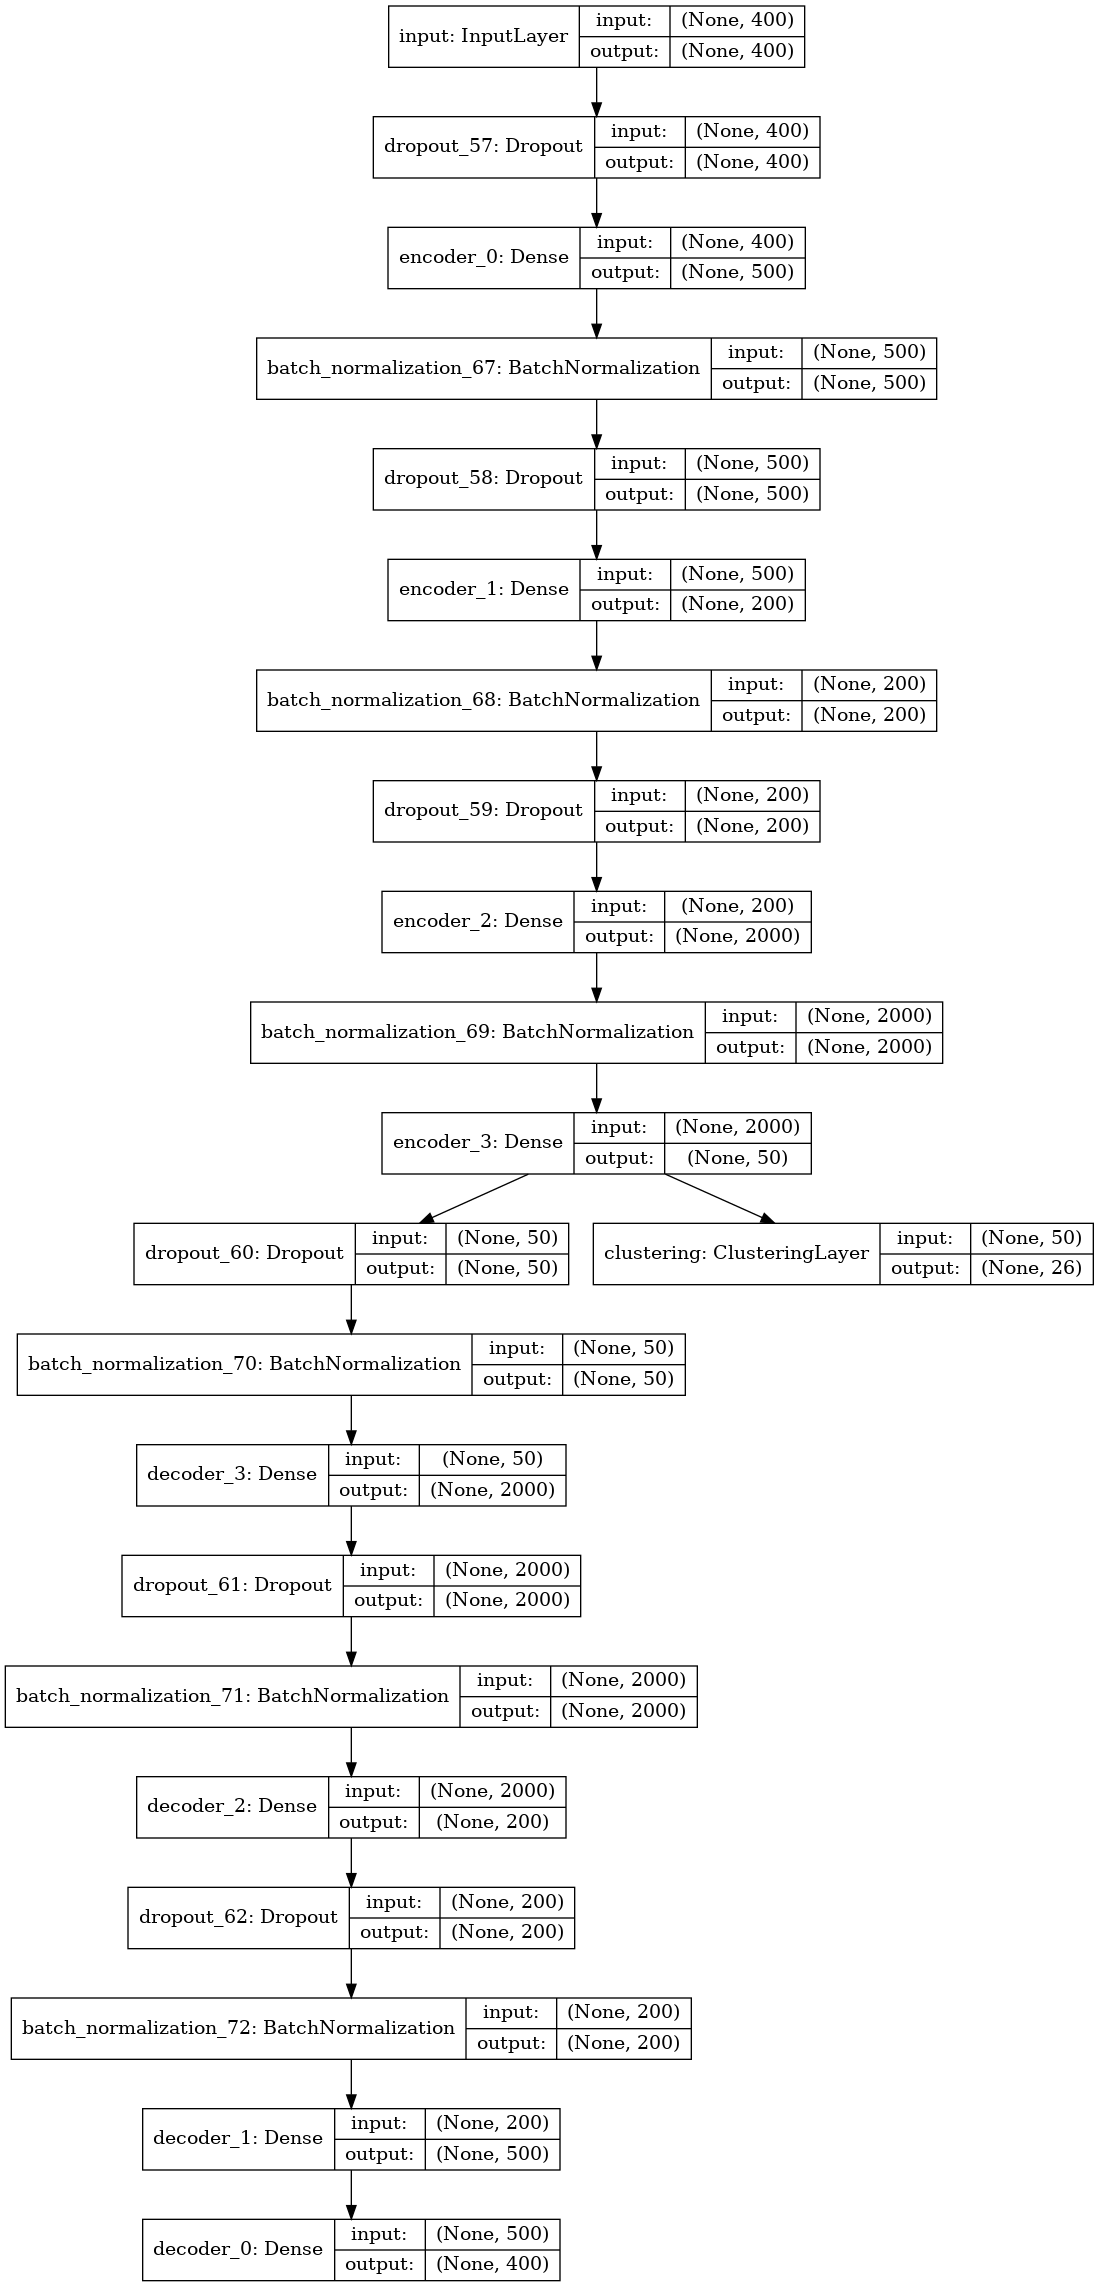
\includegraphics[width=.6\textwidth]{fig/encoder.png}
    \caption{The Structure of the DEC model}
    \label{fig:DECmodel}
\end{figure}

\clearpage

\singlespacing
\setlength\bibsep{0pt}
\bibliographystyle{plain}
\bibliography{ref}

\end{document}